\chapter{State of the art model}

\section{Spatial Resolution}

\begin{tabular}{>{\bfseries}l<{\hspace{1em}} >{\raggedleft\arraybackslash}p{5cm}}
\hline
\textbf{Model} & \textbf{Resolution} \\
\hline
Keisler \cite{keisler} & 1° * 1°\\
Pangu Weather \cite{panguweather} & 0.25° * 0.25° \\
Pangu Weather lite \cite{panguweather} & 0.25° * 0.25° \\
GraphCast \cite{graphcast} & 0.25° * 0.25° \\
GraphCast Small \cite{graphcast} & 1° * 1° \\
FuXi \cite{fuxi} & 0.25° * 0.25° \\
KARINA \cite{Karina} & 2.5° * 2.5° \\
\end{tabular}

\vspace{2em}
An interesting aspect of Keisler's approach is that he initially trained his neural network on input data with a resolution of 2 degrees for 3.5 days using a learning rate (lr) of 3e-4. Subsequently, the network was trained on data with a resolution of 1 degree for 1 day with lr=3e-5, followed by another day of training with lr=3e-6.

\section{Time Resolution}

\begin{tabular}{>{\bfseries}l<{\hspace{1em}} >{\raggedleft\arraybackslash}p{5cm}}
\hline
\textbf{Model} & \textbf{Time step (in hour)} \\
\hline
Keisler & 6 \\
Pangu Weather &  1,3,6,24 \\
Pangu Weather lite &  24 \\
GraphCast & 6 \\
GraphCast small & 6 \\
FuXi & 6 \\
KARINA & 24 \\
\end{tabular}

\vspace{2em}
Interestingly, FuXi's study builds on a comment made in the Pangu Weather paper, which notes that for a 7-day weather forecast, it is more accurate to run a 24-hour model seven times than to run a 1-hour model 168 times. This significantly reduces error accumulation. However, training a model for more than 24 hours is challenging. FuXi has developed both deterministic and ensemble versions of their model to address this challenge.

\section{Code availablity}

\begin{tabular}{>{\bfseries}l<{\hspace{1em}} >{\centering\arraybackslash}p{6cm} >{\raggedleft\arraybackslash}p{5cm}}
\hline
\textbf{Model} & \textbf{Code} & \textbf{Pre-trained}\\
\hline
Keisler & Yes \cite{keiser-github} & No \\
Pangu Weather &  Yes \cite{pangu-weather-Github} & Yes \\
Pangu Lite &  Yes \cite{pangu-weather-Github} & Yes \\
GraphCast & Yes \cite{graphcast-github} & Yes \\
GraphCast small & Yes \cite{graphcast-github} & Yes \\
FuXi & \textcolor{red}{No} \cite{fuxi-repo} & Yes \\
KARINA & \textcolor{green}{Yes} \cite{karina-code} & \textcolor{green}{Yes} \\
LAM & \textcolor{green}{Yes} \cite{neural-lam} & \textcolor{green}{Yes}
\end{tabular}

\vspace{2em}
GraphCast small has a resolution of 1°, 13 pressure levels, and trained on ERA5 data from 1979 to 2015 instead of 0.25 degree resolution, 37 pressure levels), trained on ERA5 data from 1979 to 2017.\\
Pangu Lite has only been trained and tested in 00UTC data and on 11 years instead of 39 years.

\section{Training Time with Different Models}

\begin{tabular}{>{\bfseries}l<{\hspace{1em}} >{\centering\arraybackslash}p{6cm} >{\raggedleft\arraybackslash}p{5cm}}
\hline
\textbf{Model} & \textbf{Number of GPUs} & \textbf{Training Time}\\
\hline
Keisler & 1 Nvidia A100 GPU & 5.5 days \\
Pangu Weather &  192 Nvidia Tesla-V100 GPUs & 4 * 16 days \\
GraphCast & 32 Google Cloud TPU v4 devices & 4 weeks \\
FuXi & 8 Nvidia A100 GPUs & 30 hours \\
KARINA & 4 Nvidia A100 GPUs & 12 hours \\
\end{tabular}

\newpage
\section{Keisler with Graph Neural Networks}

\subsection{Machine Learning Architecture}

\begin{figure}[ht]
\centering
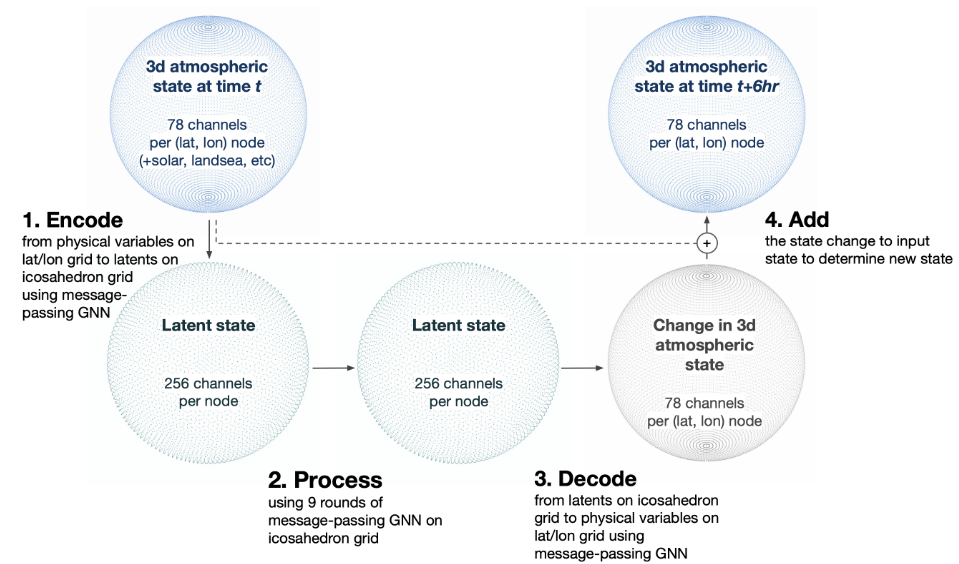
\includegraphics[width=0.9\textwidth]{media/Keisler_archi.png}
\caption{Keisler Model Learning Architecture}
\label{fig}
\end{figure}

The model employs Graph Neural Networks (GNNs) and is inspired by the approach of Pfaff et al. \cite{pfaff}. The GNN parameters are learned using historical training data (ERA5), leveraging the JAX library and two JAX-based packages: Jraph for constructing the GNN structures and Haiku for managing the neural networks themselves.

The model architecture is presented as follows: three main components - an encoder, a processor, and a decoder. The encoder maps the data from the native space (physical data on a latitude/longitude grid) to an intermediate space (abstract feature data on an icosahedral grid), while the processor handles this data in the intermediate space and the decoder maps the results back to the native space.

The use of an icosahedral grid for the intermediate representation is motivated by the fact that it provides a more uniformly distributed and efficient processing grid than the original latitude/longitude grid. The H3 package is used to define an icosahedral grid of level 2, which consists of 5,882 nodes (compared to 65,160 in the original lat/lon grid) with an angular separation of 3 degrees (approximately 330 km) between the nodes.

Each of the three components of the model is implemented as a message-passing GNN, using 2-layer MLPs with ReLU activation, LayerNorm, and 256 output channels for the neural networks.

\subsection{Data Availability}

All codes are available on this \href{https://github.com/openclimatefix/graph_weather/tree/main}{GitHub repository}.

\newpage
\section{Lam with GraphCast}

\subsection{Machine Learning Architecture}

The GraphCast system is a machine learning architecture that takes as input the two most recent states of the Earth's weather (the current time and six hours prior) and predicts the next state of the weather six hours in advance. A single weather state is represented by a latitude/longitude grid of 0.25° (721 x 1440), which corresponds to a resolution of approximately 28 x 28 kilometers at the equator, where each grid point represents a set of surface and atmospheric variables. GraphCast is autoregressive, meaning it can be "unrolled" by feeding its own predictions back into the input to generate an arbitrarily long trajectory of weather states.\\

GraphCast is implemented as a neural network architecture based on GNNs in an "encode-process-decode" configuration, with a total of 36.7 million parameters. The encoder uses a single GNN layer to map variables (normalized to zero mean and unit variance) represented as node attributes on the input grid to learned node attributes on an internal "multi-mesh" representation. The multi-mesh is a spatially homogeneous graph with high spatial resolution on the globe, defined by iteratively refining a regular icosahedron (12 nodes, 20 faces, 30 edges) six times, where each refinement divides each triangle into four smaller ones and reprojects the nodes onto the sphere.\\

The processor uses 16 unshared GNN layers to perform efficient local and long-range information propagation with few message passing steps on the multi-mesh. The decoder maps the learned features from the last layer of the processor from the multi-mesh representation to the latitude-longitude grid and predicts the output as a residual update of the most recent input state (with output normalization to achieve unit variance on the residual target).\\

During model development, 39 years (1979-2017) of historical data from the ECMWF's ERA5 reanalysis archive were used. GraphCast was trained to minimize the training objective using gradient descent and backpropagation. Training GraphCast took approximately four weeks on 32 Cloud TPU v4 devices using batch parallelism.\\

\subsection{Data Availability}

The code is available \href{https://github.com/google-deepmind/graphcast}{here}. The model is available pre-trained, as well as a smaller model with lower resolution.

\newpage
\section{Keifeng with Pangu-Weather}

\subsection{Machine Learning Architecture}

The methodology involves training deep learning networks to take reanalysis weather data as input at a given point in time and produce reanalysis weather data at a future point in time as output. The team utilized a single point in time for both input and output. The temporal resolution of the ERA5 data is 1 hour, with up to 341,880 time points in the training subset (1979-2017), constituting the amount of training data in one epoch. To mitigate the risk of overfitting, the team randomly shuffled the order of samples from the training data at the beginning of each epoch.\\

The team trained four models with lead times (the difference in time between input and output) of 1 hour, 3 hours, 6 hours, and 24 hours, respectively. Each of the four models was trained for 100 epochs, with each taking approximately 16 days on a cluster of 192 NVIDIA Tesla-V100 GPUs.\\

The architecture is known as the 3D Earth-specific transformer (3DEST). The team incorporated all the weather variables included, such as 13 layers of upper-air variables and surface variables, into a single deep network. They then performed patch embedding to reduce the spatial resolution and combined the downsampled data into a 3D cube. The 3D data is propagated through an encoder-decoder architecture derived from the Swin transformer, a vision transformer variant, which has 16 blocks. The output is divided into upper-air variables and surface variables and is resampled with patch recovery to restore the original resolution. To inject Earth-specific priorities into the deep network, the team designed a position bias (a mechanism for encoding the position of each unit) to replace the original relative position bias of Swin. This modification increases the number of bias parameters by a factor of 527, with each deep 3D network containing approximately 64 million parameters.\\

The lead time of a medium-range weather forecast is 7 days or more. This prompted the team to call the base models (with lead times of 1 hour, 3 hours, 6 hours, or 24 hours) iteratively, using each predicted result as input for the next step. To reduce cumulative forecast errors, they introduced a hierarchical temporal aggregation, a 'greedy' algorithm that always calls the model with the largest possible lead time. Mathematically, this significantly reduces the number of iterations. For example, if the lead time were 56 hours, the team would run the 24-hour forecast model 2 times, the 6-hour forecast model 1 time, and the 1-hour forecast model 2 times (Figure 1b). Compared to FourCastNet, which uses a fixed 6-hour forecast model, the team's method is faster and more accurate.\\

\subsection{Data Availability}

The code is available but currently under review. The pre-trained model is also available, along with a lite version that has a 24-hour step and has been tested only on 00 UTC.\\

\newpage
\section{Chen with FuXi}

The aim of this paper is to mitigate the error in forecasts due to the low-step model used for long-range predictions (10 days).

\subsection{Machine Learning Architecture}

\begin{figure}[ht]
\centering
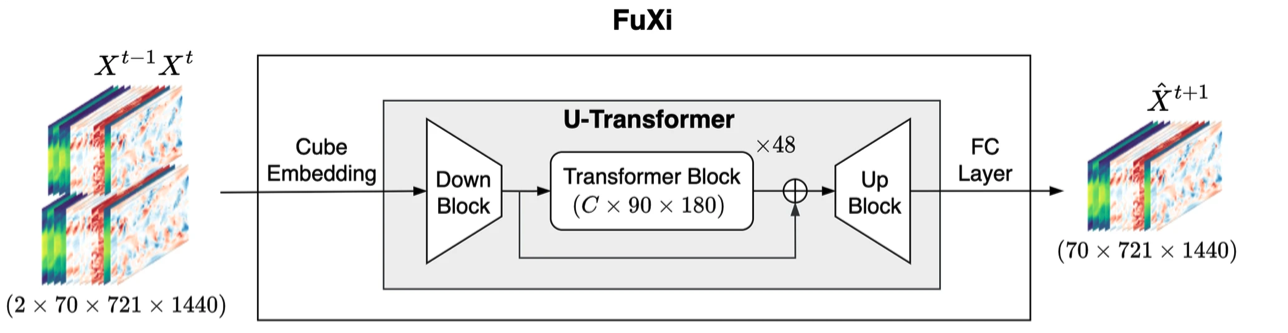
\includegraphics[width=0.9\textwidth]{media/FuXi_archi.png}
\caption{FuXi model learning architecture.}
\label{fig}
\end{figure}


\subsection{Data Availability}

The code for the model is available, albeit unreviewed. The pre-trained model is also available.

\newpage
\section{Cheon with KARINA}

KARINA is a machine learning model for global weather prediction that aims to be computationally efficient, particularly during training. It required 4 NVIDIA A100 GPUs for less than 12 hours of training. However, the model has a low resolution of 2.5 degrees. It utilizes 66 parameters, including 6 surface parameters and 5 atmospheric parameters, across 12 vertical isobaric layers from the surface to the lower stratosphere. The tensor has a dimension of 7214466. The low resolution is considered by the authors to be an effective means of extracting global patterns while smoothing noise.\\

\subsection{ML Architecture}

The model employs a ConvNext architecture with two innovations: SENet for dynamic parameter recalibration and the introduction of geocyclic padding to preserve continuity at 0° and 360°.\\

Squeeze-and-Excitation Networks (SENet) enable the model to focus on the most relevant features and meteorological variables through channel-wise recalibration.\\

Geocyclic Padding: Geocyclic padding handles the spherical topology by performing circular padding of the longitudinal edges and reorganizing the polar regions. This maintains geographic continuity.\\

\subsection{Data Availability}

The paper has been available for one month and has not yet been published in an official journal. The code has just been made available \href{https://github.com/jmj2316/KARINA/}{on this GitHub repository}.\\

\subsubsection{\href{https://github.com/jmj2316/KARINA/blob/main/networks/karina.py}{KARINA.py}}

Let's analyze the code named KARINA.py in detail:
This code is the body of the implementation of their CNN presented in the paper.\\

We can start with the functions:\\

\begin{itemize}
\item \textbf{SELayer(nn.Module)}: This class defines the Squeeze-and-Excitation Layer, which is the channel attention layer. An attention layer allows a CNN to "improve the representation of features." This class defines two functions:
\begin{enumerate}
\item \textbf{Init}: The class constructor takes two arguments: channel (the number of channels) and reduction, which I believe reduces the dimensionality of the data by a factor of 16. In this constructor, we find: mean pooling on the input data, a fully connected layer (all nodes in the layer connect to all nodes in the next layer) with ReLu and Sigmoid activation functions.
\item \textbf{Forward}: Applies mean pooling and then the fully connected layer to y, then multiplies the input tensor x by y, which is resized to match the size of x.
\end{enumerate}
\item \textbf{GeoCyclicPadding}: This class allows the innovation presented in the paper, i.e., to create a tensor that represents the constraint of a spherical domain. (I won't go into detail for now)
\item \textbf{Block}
\begin{enumerate}
\item \textbf{Init}: The class constructor with three arguments: dim, the input dimension, droppath, the dropout rate set to zero, and therefore this function is never used (i.e., the input tensor is transmitted without modification). It can prevent overfitting in some cases, but it does not seem to be used here. Otherwise, the rest of the function is intended to apply \textit{SELayer and GeoCyclic Padding}
\item \textbf{Forward}: The way x is propagated through a network.
\end{enumerate}
\item \textbf{ConvNext}:
\begin{enumerate}
\item \textbf{Init}: The class constructor with four arguments: the number of input channels (in chans), the number of output classes (num classes), the depths of the different blocks (depths), and the dimensions of the different blocks (dims). It initializes the downsampling layers (downsample layers) and the stages of the network using the Block defined above.
\item \textbf{init weights}: As the name suggests, it initializes the weights.
\item \textbf{forward features and forward}: The way x is propagated through the network.
\end{enumerate}
\item \textbf{Layer Norm}: As the name suggests, this class is used to normalize the network, layer by layer. It uses the layer norm function of PyTorch.
\item \textbf{KARINA}:
\begin{enumerate}
\item  \textbf{init} 5 arguments : the size of the image (img size), the number of input channels (in chans), the number of output channels (out chans), the depths of the different blocks (depths) and the dimensions of the different blocks (dims)
\item \textbf{forward} it propagates the network in convnext.
\end{enumerate}
\item \textbf{Main}: Defines the input and passes it through the model.
\end{itemize}

\subsubsection{\href{https://github.com/jmj2316/KARINA/blob/main/train_KARINA.py}{train-KARINA.py}}

Let's analyze in detail how the model is trained. \textbf{TO BE DONE LATER}\\

\begin{itemize}
\item \textbf{Set seed(seed)}: This function aims to define a SINGLE random number generator and thus to have reproducibility of results (by performing the same operation, we will get the same result). In this function, we define the "seed" for PyTorch CPU and GPU, for numpy random and classic random, for object hashing (not well understood here the interest). We define cuDNN as deterministic: convolution operations are therefore deterministic and reproducible. And we disable the \textbf{benchmark} option, which seems to automatically select convolution algorithms, and therefore, once again, in the interest of result reproducibility, we disable this option.
\end{itemize}

\newpage
\section{Limited Area Modelling}

This section follows up on a discussion initiated by Prof. Myoshi in Vienna \cite{Raynaud2024}. Upon conducting research, I came across a publication by Joel Oskarsson et al. \cite{LAM}. To deepen my understanding of this domain, I should read this \href{https://www.researchgate.net/publication/349484799}{chapter}.\\

The title of the article is "Graph-based Neural Weather Prediction for Limited Area Modeling." In this article, the authors present an implementation of a neural weather prediction system based on graph theory. The article describes three models: GC-LAM, 1L-LAM, and HI-LAM.\\

The first two models, GC-LAM and 1L-LAM, are direct implementations of the GraphCast model. In GraphCast, the boundaries of each node's domain have different resolutions, enabling the propagation of long-range physical phenomena while maintaining precision for local phenomena.\\

HI-LAM introduces an innovation by proposing different node architectures adapted to various resolutions. This approach addresses the problem of nodes having less information than others. In HI-LAM, all nodes receive the same information, eliminating certain artifacts along the edges of the nodes.\\

\begin{figure}[ht]
\centering
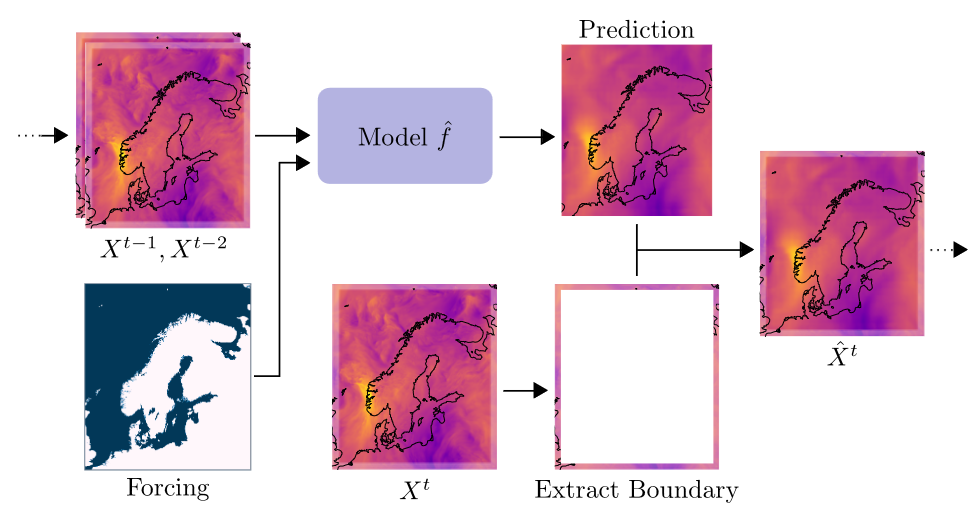
\includegraphics[width=0.9\textwidth]{media/LAM_Boundary-Forcing.png}
\caption{Boundary forcing in the case of a LAM}
\label{fig}
\end{figure}

A specific consideration is how the boundary conditions are obtained. To address this issue, before each iteration, an expanded domain is given to the algorithm to define the forcing (see figure \ref{fig}). One question that arises is whether this expanded domain is sufficient, or if a global model should be provided to the system for more relevant predictions. Furthermore, in an operational context, we would be required to use a global model to extract this information at each time step. Therefore, a low-resolution global model coupled with a high-resolution local model would be advantageous.

